% !TEX root = ./informe.tex

\section{Problema 1}

\subsection{Explicación}

Tenemos ciudades conectadas por rutas bidireccionales, donde algunas rutas tienen la particularidad de ser $premium$. El problema es calcular el camino minimo desde ciudad $origen$ hacia una $destino$, pasando por a lo sumo $k$ rutas premium (devolviendo -1 de no existir solución). \\

La particularidad de este problema es que un algoritmo greedy como el de Dijkstra no parecería funcionar. El motivo es que, dado un camino premium, no puedo saber si el hecho de tomarlo resulta en un callejón sin salida. Esto implica que la distancia de un nodo puede quedar actualizada con el valor de un camino que no puede llegar al destino. Esto nos imposibilita considerar caminos hacia ese nodo pesos mayores, pero que por tener menos caminos premium terminan siendo mejor opción. \\

La estrategia general va a ser plantearse $k$ versiones para cada nodo, donde cada uno representa un \textit{estado} distinto. Habiendo hecho esta separación, simplificamos los roles de los ejes premium, y nos permite aplicar el algoritmo de Dijkstra, con algunas leves variaciones.

\subsection{Correctitud}
Queremos representar cada ciudad como un vértice y cada ruta como una arista con el objetivo de calcular el camino mínimo entre el origen y el destino mediante algún algoritmo conocido y probado para este propósito. Llamaremos a este grafo $G_0$\\

El principal inconveniente de este planteo es el modelado de las rutas premium, las cuales (y según el valor de $k$) pueden restringir las aristas disponibles para el cálculo del camino mínimo a medida que se recorran vértices utilizando estas rutas.\\

Es importante notar que existen diferentes estados para cada vértice, a modo de ejemplo, para $k=1$ y ningún camino premium recorrido, los vértices pueden utilizar cualquier arista, por lo que si $v_i$ es adyacente a $v_j$ para el input original, entonces seguirá siéndolo. Este no es el caso si se ha recorrido un camino premium, en este caso si la arista $(v_i, v_j)$ fuera premium entonces $v_i$ ahora no es adyacente a $v_j$. En conclusión, los estados de los vértices dependen de la cantidad de aristas premium recorridas.\\

Siendo $K$ la máxima cantidad de caminos premium a recorrer, cada vértice puede tener hasta $K$ estados diferentes. Se resuelve modelar un digrafo $G_1$ y representar a cada estado como un vértice $v_i^k$ en el cual sus aristas responden a las siguientes reglas:
\begin{itemize}
	\item Si $(v_i,v_j) \in E_{G_0} \land (v_i,v_j) \notin premium \Rightarrow (v_i^k,v_j^k) \in E_{G_1} \land (v_j^k,v_i^k) \in E_{G_1}$
	\item Si $(v_i,v_j) \in E_{G_0} \land (v_i,v_j) \in premium \land k < K \Rightarrow (v_i^k,v_j^{k+1}) \in E_{G_1}$
\end{itemize}
En este modelo no es posible recorrer más de $K$ aristas premium, dado que cada vez que se recorre cualquier premium se pasa de un vértice $k$ a uno $k+1$ (exceptuando $k=K$ en el cual no existe vértice premium para ningún $v^k$) y sólo existen $K$ estados disponibles.\\\\
Además, al tratarse de un simple digrafo con aristas positivas, se puede calcular el camino mínimo entre el origen y todos los demás vértices utilizando el algoritmo de Dijkstra, para luego obtener $min(v_{destino}^k \forall k)$, la distancia mínima entre origen y destino pasando por a lo sumo $k$ aristas premium. Siendo el origen en $v_i^0$ para algún $i$ especificado en la entrada, esto es así porque el vértice de origen no recorrió ninguna arista, en particular ninguna arista premium, por lo que pertenece al estado $k=0$, además los vértices $\{v_j^0,v_j^1,...,v_j^k\}$ representan al vértice destino para un $j$ especificado en la entrada, siendo $k$ la cantidad de aristas premium recorridas, por lo que al aplicar dijkstra sobre $G_1$ empezando por el origen, tendremos todas las distancias de este hacia los vértices destino (de distintos $k$), entre los cuales hay que elegir el que tenga una distancia mínima. \\

\subsection{Pseudocodigo}

(Ver notas debajo del pseudocodigo las referencia de significados de las variables)
% Vamos a utilizar como entrada en nuestro algoritmo las siguientes variables:

\begin{algorithm}[H]
% \label{ej3}         % and a label for \ref{} commands later in the document
\begin{algorithmic}
\Function{Resolver}{}    \Comment{$\mathbf{\mathcal{O}(n^2*k^2)}$}
	\State $visitado \gets$ InitSecuenciaEnFalso($n*(k+1)+1$)    \Comment{$\mathcal{O}(n*k)$}
	\State $dist \gets$ InitSecuenciaEnInfinito($n*(k+1)+1$)    \Comment{$\mathcal{O}(n*k)$} \\

	\State $s = origen$    \Comment{$\mathcal{O}(1)$}
	\For{$w \in [1..n]$}    \Comment{$\mathcal{O}(n)$}
		\If{$matrizAdy[s][w] \not = 0$}    \Comment{$\mathcal{O}(1)$}
			\If{$esPremium[s][w]$}    \Comment{$\mathcal{O}(1)$}
				\If{$k > 0$}    \Comment{$\mathcal{O}(1)$}
					\State $dist[w+n] \gets matrizAdy[s][w]$    \Comment{$\mathcal{O}(1)$}
				\EndIf
			\Else
				\State $dist[w] \gets matrizAdy[s][w]$    \Comment{$\mathcal{O}(1)$}
			\EndIf
		\EndIf
	\EndFor \\

	\State $dist[s] \gets 0$    \Comment{$\mathcal{O}(1)$}
	\State $visitado[s] \gets True$    \Comment{$\mathcal{O}(1)$} \\

	\State $finalizado \gets False$    \Comment{$\mathcal{O}(1)$}

	\While{$\neg finalizado$}    \Comment{$\mathcal{O}(n*k)$\hyperref[whilejust]{$^{[1]}$}\label{whileback}}
		\State $v \gets -1$    \Comment{$\mathcal{O}(1)$}
		\State $minDist = \infty$    \Comment{$\mathcal{O}(1)$}
		\For{$u \in [1..n*(k+1)]$}    \Comment{$\mathcal{O}(n*k)$}
			\If{$\neg visitado[u] \land dist[u] < minDist$}    \Comment{$\mathcal{O}(1)$}
				\State $v \gets u$    \Comment{$\mathcal{O}(1)$}
				\State $minDist \gets dist[u]$    \Comment{$\mathcal{O}(1)$}
			\EndIf
		\EndFor

		\If{$minDist = \infty$}    \Comment{$\mathcal{O}(1)$}
			\State $finalizado \gets True$    \Comment{$\mathcal{O}(1)$}
			\State \textbf{continue} \Comment{$\mathcal{O}(1)$}
		\EndIf \\

		\State $visitado[v] \gets True$    \Comment{$\mathcal{O}(1)$}
		\State $nivel \gets (v-1)/n$    \Comment{$\mathcal{O}(1)$}
		\State $vOriginal \gets v - n * nivel$     \Comment{$\mathcal{O}(1)$} \\

		\For{$w \in [1..n]$}    \Comment{$\mathcal{O}(n)$}
			\If{$matrizAdy[vOriginal][w] \not = 0$}    \Comment{$\mathcal{O}(1)$}
				\If{$esPremium[vOriginal][w]$}    \Comment{$\mathcal{O}(1)$}
					\If{$nivel = k$}    \Comment{$\mathcal{O}(1)$}
						\State \textbf{continue}    \Comment{$\mathcal{O}(1)$}
					\EndIf
					\State $vecinoPremium \gets w + (nivel+1) * n$    \Comment{$\mathcal{O}(1)$}
					\If {$\neg visitado[vecinoPremium]$}    \Comment{$\mathcal{O}(1)$}
						\If{$dist[vecinoPremium] > dist[v] + matrizAdy[vOriginal][w]$}    \Comment{$\mathcal{O}(1)$}
							\State $dist[vecinoPremium] = dist[v] + matrizAdy[vOriginal][w]$    \Comment{$\mathcal{O}(1)$}
						\EndIf
					\EndIf
				\Else
					\State $vecinoComun \gets w + nivel*n$    \Comment{$\mathcal{O}(1)$}
					\If {$\neg visitado[vecinoComun]$}    \Comment{$\mathcal{O}(1)$}
						\If{$dist[vecinoComun] > dist[v] + matrizAdy[vOriginal][w]$}    \Comment{$\mathcal{O}(1)$}
							\State $dist[vecinoComun] = dist[v] + matrizAdy[vOriginal][w]$    \Comment{$\mathcal{O}(1)$}
						\EndIf
					\EndIf
				\EndIf
			\EndIf
		\EndFor
	\EndWhile \\

	\State $distanciaMinima \gets \infty$    \Comment{$\mathcal{O}(1)$}

	% @jonno: que tal asi?
	\For{$index \in [0 .. (k+1)]$}    \Comment{$\mathcal{O}(k)$}
		\State $i \gets$ $destino + index * n$ \Comment{$\mathcal{O}(1)$}
		\If{$dist[i] < distanciaMinima$}    \Comment{$\mathcal{O}(1)$}
			\State $distanciaMinima \gets dist[i]$    \Comment{$\mathcal{O}(1)$}
		\EndIf
	\EndFor \\

	% \For{$i \in [destino, destino + n, destino + 2n \, .. \, n*(k+1)]$}    \Comment{$\mathcal{O}(k)$}
	% 	\If{$dist[i] < distanciaMinima$}    \Comment{$\mathcal{O}(1)$}
	% 		\State $distanciaMinima \gets dist[i]$    \Comment{$\mathcal{O}(1)$}
	% 	\EndIf
	% \EndFor \\

	\If{$distanciaMinima = \infty$}    \Comment{$\mathcal{O}(1)$}
		\State \Return $-1$    \Comment{$\mathcal{O}(1)$}
	\Else
		\State \Return $distanciaMinima$    \Comment{$\mathcal{O}(1)$}
	\EndIf
\EndFunction

\end{algorithmic}
\end{algorithm}
% \todo[inline]{En el último for hago el 'step = n' de una forma rara, ideas bienvenidas}

Referencias de variables parra el pseudocódigo:

\begin{itemize}
	\item $n$: La cantidad de ciudades
	\item $m$: La cantidad de aristas
	\item $k$: La máxima cantidad de rutas premium posibles de recorrer
	\item $origen$: La ciudad origen
	\item $destino$: La ciudad destino
	\item $matrizAdy$: El grafo de entrada representado con matriz de adyacencia.
	\item $esPremium$: La matriz de booleanos que indica si una ruta es premium o no
\end{itemize}

\subsection{Complejidad}

\begin{itemize}
	\item Leer el input es O($n^2$): Construimos dos matrices de O($n^2$) elementos parseando la entrada.
	\item Inicializar estructuras del algoritmo es O($n*k$): Recorremos las O($n*k$) ciudades actualizando las distancias de los vecinos de $origen$
	\item Visitar todos los nodos llevando a cabo el algoritmo de Dijkstra es O($n*k$): En cada iteración marco el nodo actual como $visitado$, y tengo como máximo $n*k$ nodos (por esta razón vale  \label{whilejust}\hyperref[whileback]{$[1]$} \textit{-referencia en pseudocodigo-})
	\item Buscar el nodo de menor distancia es O($n*k$):  Buscamos linealmente la mínima distancia entre O($n*k$) nodos
	\item Actualizar la distancia de los vecinos de una ciudad es O($n$): Podemos reducir los potenciales vecinos a O($n$) porque sabemos que un nodo sólo puede tener un camino hacia nodos de su mismo $nivel$ o de un $nivel$ superior
\end{itemize}

$$Total:  O(n^2) + O(n*k) + O(n*k) * (O(n*k) + O(n)) = O(n^2*k^2) $$

\subsection{Experimentos}

En todos lo experimentos, para cada tamaño se corrió el programa 50 veces, guardando el tiempo de cada ejecución. Para elegir un valor representativo de la muestra se tomó el promedio del tiempo para cada tamaño. \\

En el primer experimento, vemos como se comporta el programa a medida que aumentamos la cantidad de nodos, para diferentes porcentajes de aristas premiums.

Las aristas son generadas aleatoriamente, y el K (\textit{máxima cantidad de premiums que pueden usarse}) tambien es aleatorio, entre 0 y la cantiad de aristas totales. \\

Si no hay aristas premium, solo se recorrerá un unico \textit{nivel} de cada nodo, por lo que se ejecuta es el algoritmo de Dijkstra clásico.

En caso de existir alguna premium, se recorren tambien diferentes \textit{niveles} de un mismo nodo. Es decir, si \textit{v} es un nodo, se recorre \textit{v}, \textit{v pasando por 1 premium}, \textit{v pasando por 2 premiums}, etc, por lo que es esperable que los tiempos de ejecucion sean muchos mayores en estos casos. \\

{\centering
  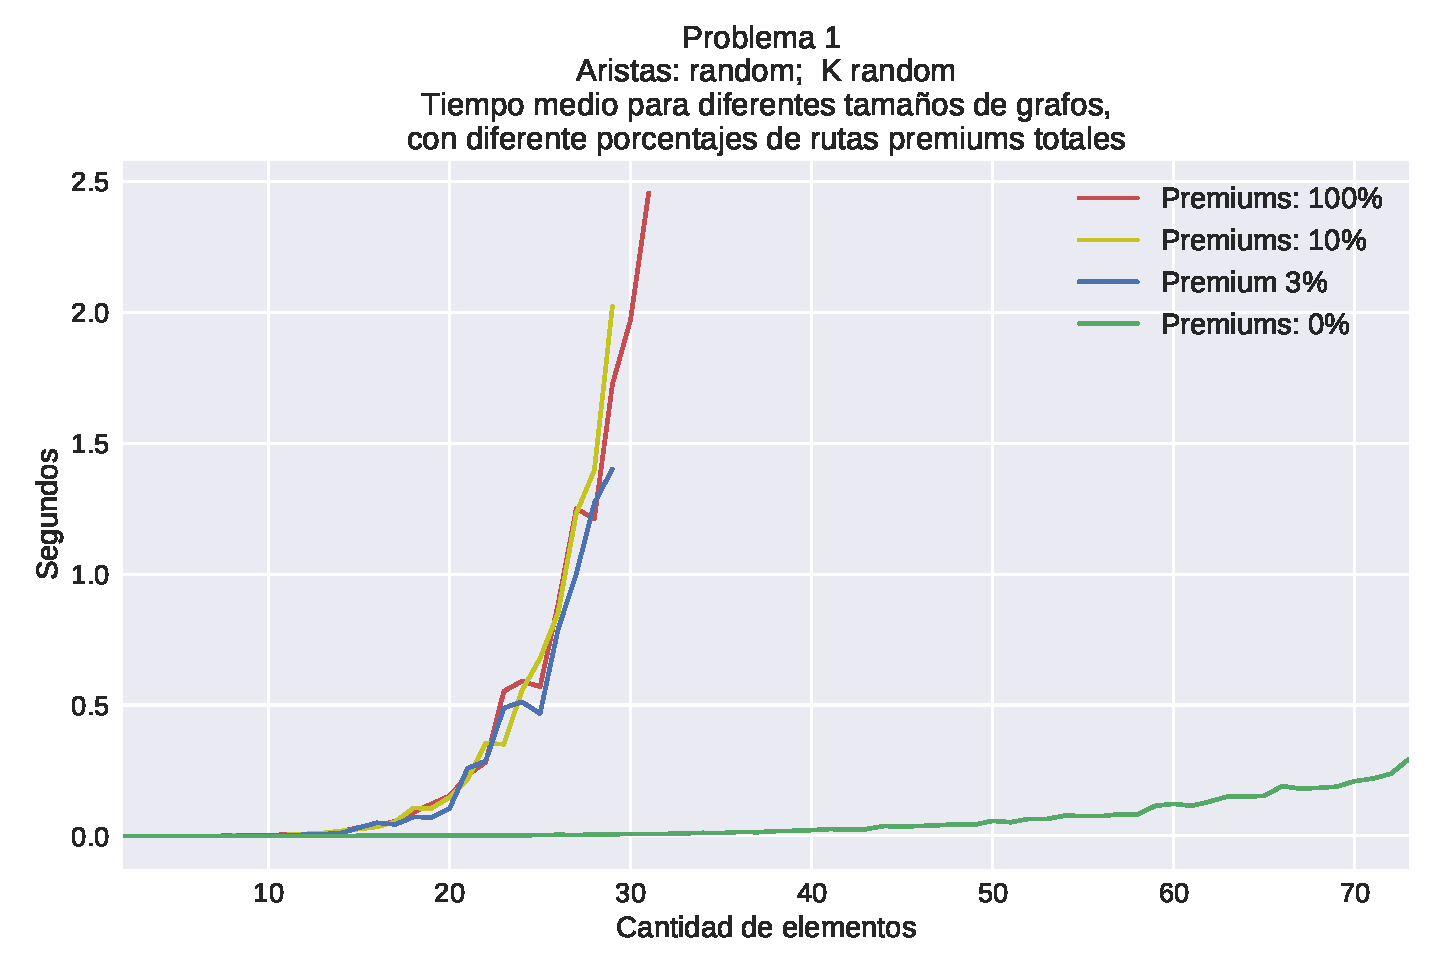
\includegraphics[width=0.9\textwidth]{imagenes/problema1/todo_random_bis.pdf} \\
}

Dado que hay varias variables que son dejadas al azar y las curvas no son muy regulares, veamos que pasa cuando tomamos un $K$ fijo (con respecto a $N$). Tomamos $K$ tal que sea siempre la mitad de la cantidad de nodos, es decir $K = N/2$. \\

Observamos que en lineas generales sucede lo mismo en el caso anterior, con la diferencia en que en este caso las curvas son suaves. Cuando no hay premiums siempre es mas eficiente calcular la respuesta. \\

{\centering
  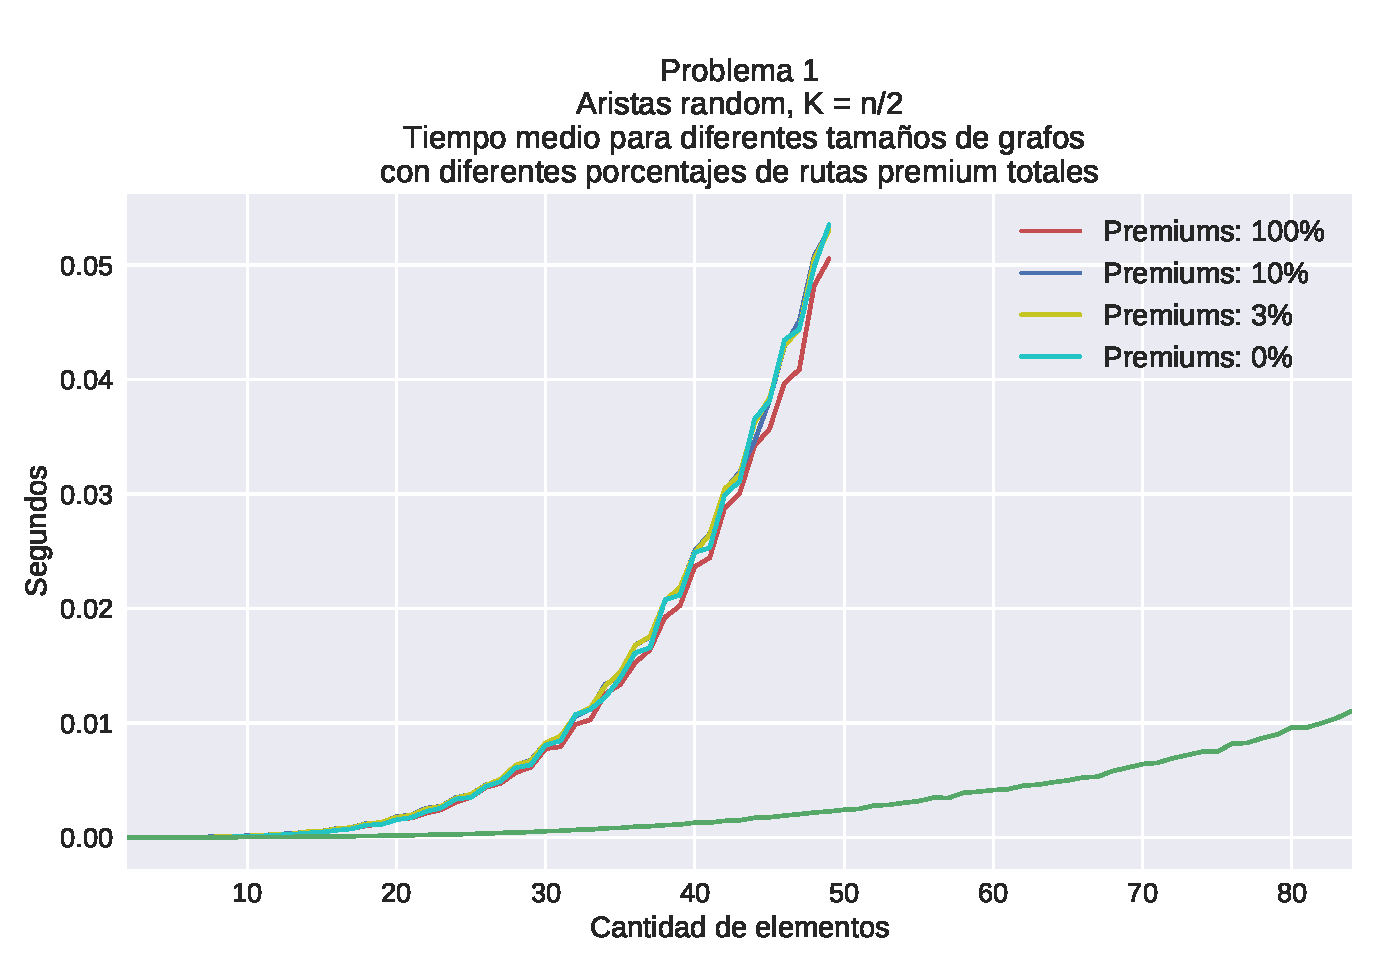
\includegraphics[width=0.9\textwidth]{imagenes/problema1/kfijo.pdf} \\
}

Veamos que sucede cuando dejamos el $N$ fijo y vamos variando el $K$. Si no hay rutas premium sigue siendo lo mas eficiente por las mismas razones que antes. \\

Cosa interesante: si el 100\% de las aristas son premiums, puede verse una \textit{pequeña} mejora con respecto a los otros porcentajes. Esto es porque \todo{ver}


{\centering
  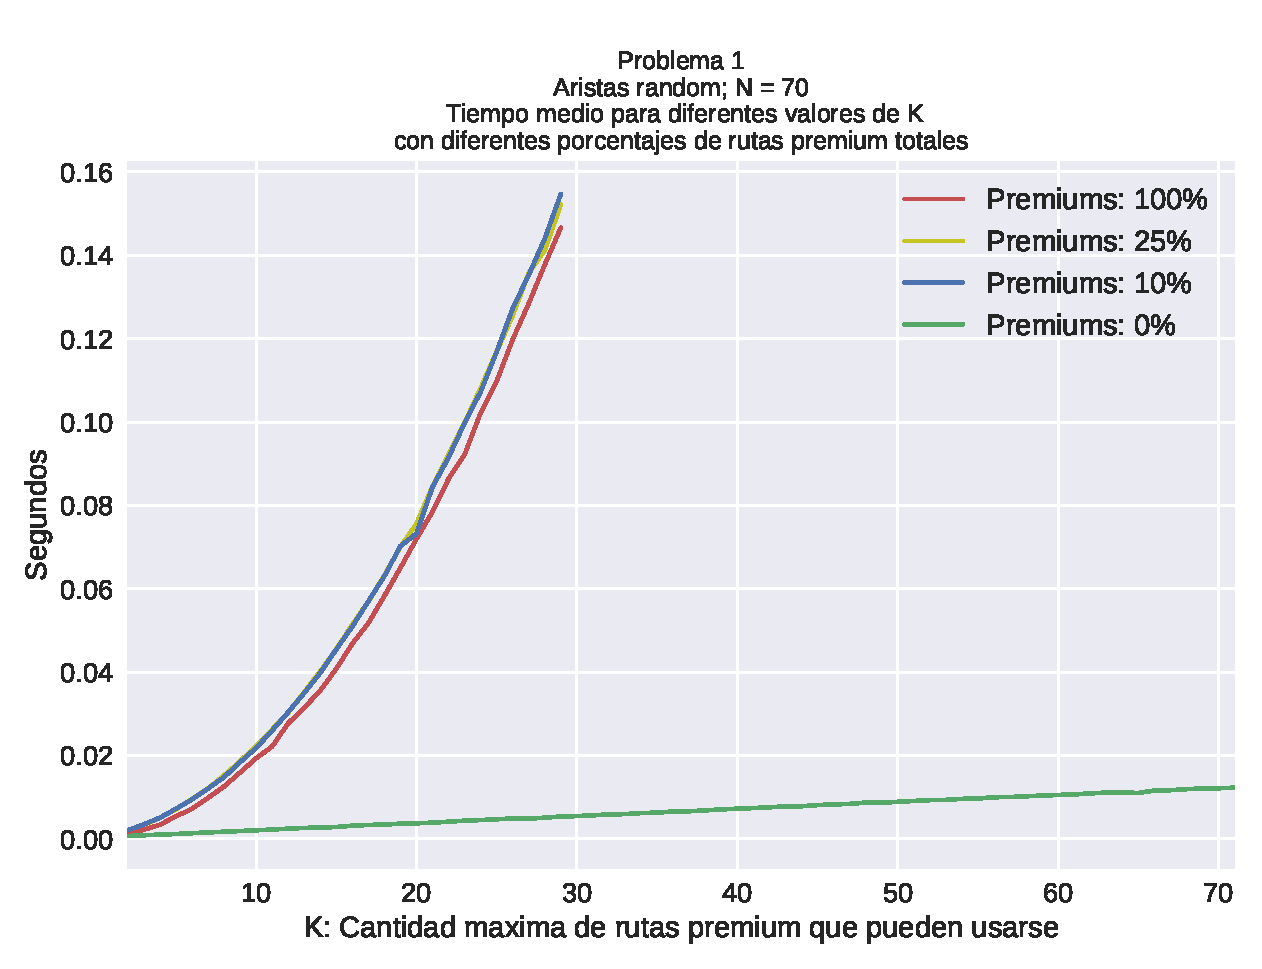
\includegraphics[width=0.9\textwidth]{imagenes/problema1/nfijo.pdf} \\
}

\todo{conclusion}
en conclusion, siempre es mejor cuando no hay ninguna premium porque blablaba
